% Created 2022-05-08 Sun 11:48
% Intended LaTeX compiler: pdflatex
\documentclass[11pt]{article}
\usepackage[utf8]{inputenc}
\usepackage[T1]{fontenc}
\usepackage{graphicx}
\usepackage{longtable}
\usepackage{wrapfig}
\usepackage{rotating}
\usepackage[normalem]{ulem}
\usepackage{amsmath}
\usepackage{amssymb}
\usepackage{capt-of}
\usepackage{hyperref}
\author{Mitch Richling}
\date{YYYY-MM-DD FIXME}
\title{TITLE FIXME}
\hypersetup{
 pdfauthor={Mitch Richling},
 pdftitle={TITLE FIXME},
 pdfkeywords={KEYWORDS FIXME},
 pdfsubject={DESCRIPTION FIXME},
 pdfcreator={Emacs 28.1 (Org mode 9.5.2)}, 
 pdflang={English}}
\begin{document}

\maketitle
\begin{center}
\begin{tabular}{rl}
\textbf{Author:} & \emph{Mitch Richling}\\
\textbf{Updated:} & \emph{2022-05-08 11:48:20}\\
\textbf{Generated:} & \emph{2022-05-08 11:48:24}\\
\end{tabular}
\end{center}
Copyright 2022 Mitch Richling. All rights reserved.

\setcounter{tocdepth}{5}
\tableofcontents

\section{Math}
\label{sec:orgcba23b3}

Here is some math \(5+3^4\).

Reminder: toggle inline preview of an expression with C-c C-x C-l

Here is some display math $$\sum 4$$

\section{Markup}
\label{sec:org1776124}

\subsection{Inline stuff}
\label{sec:org161efae}

Some \textbf{bold} text.

Some \emph{italics} text.

Some \uline{underlined} text.

Some \texttt{verbatim} text.

Some \texttt{code} text.

Some \sout{strike-through} text.

\subsection{Structural stuff}
\label{sec:org1de6d92}

\subsubsection{Special Paragraphs}
\label{sec:org2138ffb}

Here we have a quote:
\begin{quote}
A human being is a part of a whole, called by us \uline{universe}, a part limited in time and space. He experiences himself, his thoughts and feelings as something
separated from the rest\ldots{} a kind of optical delusion of his consciousness. This delusion is a kind of prison for us, restricting us to our personal desires
and to affection for a few persons nearest to us. Our task must be to free ourselves from this prison by widening our circle of compassion to embrace all
living creatures and the whole of nature in its beauty. -- Albert Einstein
\end{quote}

We can also keep newlines intact in an indented paragraph:
\begin{verse}
Whales Weep Not!\\
\vspace*{1em}
They say the sea is cold, but the sea contains\\
the hottest blood of all, and the wildest, the most urgent.\\
\ldots{}\\
\vspace*{1em}
\hspace*{3em}-- D.H. Lawrence\\
\end{verse}

We can have a "verbatim" section with an "EXAMPLE" block.
\begin{verbatim}
     Here is some text.
Note that
 everything is    just as typed.
\end{verbatim}

\subsubsection{Tables}
\label{sec:org66c0139}

\paragraph{With formatting \& a formula}
\label{sec:orgf9e2d12}

\begin{table}[htbp]
\caption{A formatted table}
\centering
\begin{tabular}{l|l|rl}
\hline
col 1 & col 2 & col 3 & Col 4\\
\hline
another & bit & 1 & 1.00\\
a & b & 2 & 4.00\\
\hline
\end{tabular}
\end{table}

\paragraph{Tables used to hold data}
\label{sec:orgfef9e43}

We can use tables to hold data for other blocks to read in the document.  The
section \ref{sec:org09ef2fc} shows how to access
the table below from R.  Note some specifics for R:
\begin{itemize}
\item We have no "top line" on the table -- otherwise the row of titles is not recognized!!
\item Spaces in column titles are transformed into periods for \texttt{data.frame} column names.
\item Empty data cells will be \texttt{NA} in the \texttt{data.frame}
\item Non-numeric columns will be "characters" not "factors"
\end{itemize}

\begin{table}[htbp]
\label{tab:orge4ece1c}
\centering
\begin{tabular}{llrr}
factor 1 & factor 2 & value 1 & value 2\\
\hline
a & z & 1 & 5\\
a & x & 2 & 6\\
a & y & 3 & 7\\
b & x & 4 & \\
\end{tabular}
\end{table}

\subsubsection{Lists}
\label{sec:org71d1d4a}

Here is itemized list:

\begin{itemize}
\item first
\item second
\item third
\end{itemize}

Here is enumerated list:

\begin{enumerate}
\item First
\item Second
\item Third
\end{enumerate}

A bit of both:

\begin{enumerate}
\item First
\item Second
\begin{itemize}
\item first
\item second
\item third
\end{itemize}
\item Third
\end{enumerate}

\subsection{Todo/action items}
\label{sec:org4f63d53}

\subsubsection{{\bfseries\sffamily TODO:NEW} This is a todo}
\label{sec:org16f0b8e}

\subsubsection{ACTION:DONE This is an action item -- work speak. ;)}
\label{sec:org22f8adf}
\noindent\textbf{CLOSED:} \textit{[2015-11-01 Sun 22:36] } \textbf{DEADLINE:} \textit{<2015-11-01 Sun>}\\

\subsubsection{ACTION:NEW This is an item with sub-items [1/2]}
\label{sec:orge7f1aca}
\paragraph{ACTION:DONE A subitem}
\label{sec:org7dc74e3}
\noindent\textbf{CLOSED:} \textit{[2015-11-01 Sun 22:39]}\\
\paragraph{ACTION:NEW Another subitem}
\label{sec:org92af14c}

\subsubsection{ACTION:NEW Here is an action item with list compoents [2/3]}
\label{sec:orgebcfa61}
\noindent\textbf{DEADLINE:} \textit{<2015-11-03 Tue> } \textbf{SCHEDULED:} \textit{<2015-11-01 Sun>}\\
\begin{itemize}
\item[{$\square$}] Step 1
\item[{$\boxtimes$}] Step 2
\item[{$\boxtimes$}] Step 3
\end{itemize}

\section{Images}
\label{sec:orgd0adabf}

\subsection{PDFs in \LaTeX{} and Raster Image in HTML}
\label{sec:orgaaa27bd}

In this Section you will see one image.  A PNG for HTML, and a PDF for \LaTeX{}!

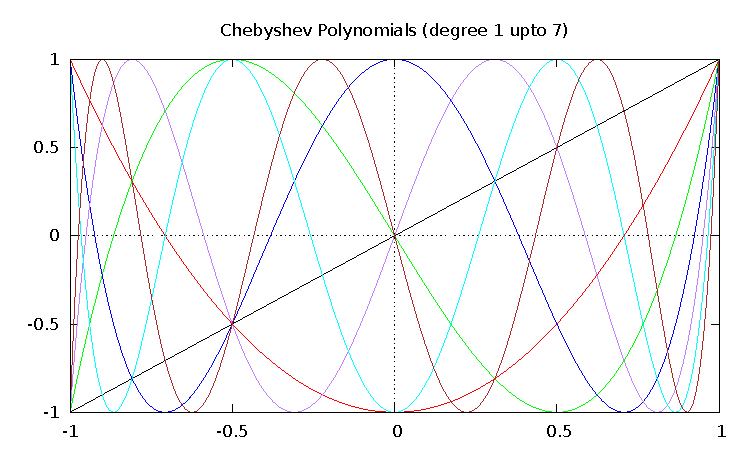
\includegraphics[width=4in]{example.pdf}

\subsection{Links to images and converting PDFs to high quality raster images}
\label{sec:org67708ac}

Here we have a pretty graph (in a PNG file):

\begin{center}
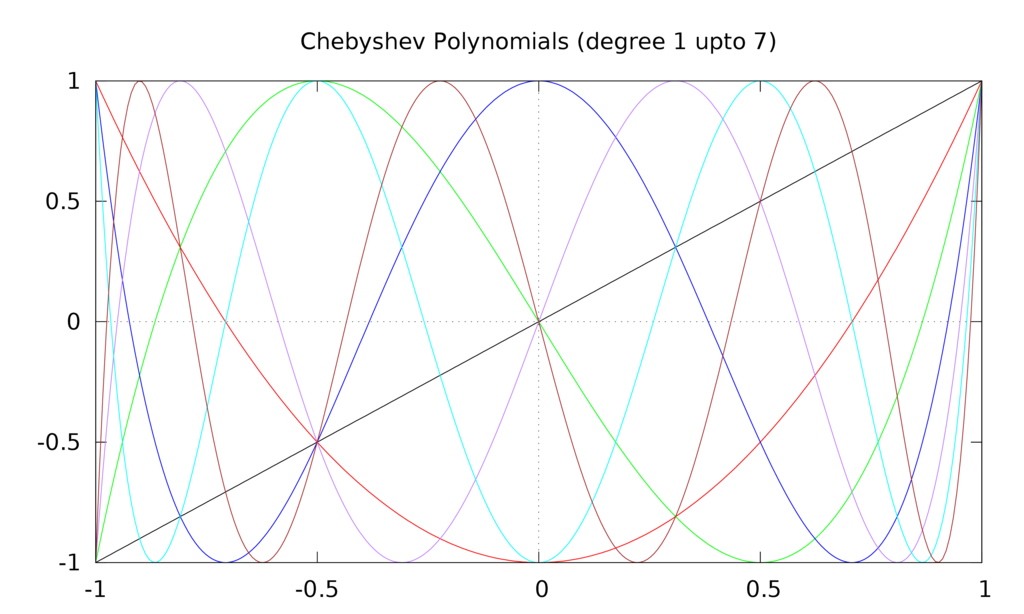
\includegraphics[width=.9\linewidth]{example.png}
\end{center}

The above file was generated from a high quality PDF file: \href{example.pdf}{example.pdf}. Note that the link in the previous sentence is a link in both HTML and \LaTeX{} because
the link has a 'display text' component.

The conversion was done like so:

\begin{verbatim}
convert -density 600 -resize 1024 -background white -flatten example.pdf example.png
\end{verbatim}

\section{Including external code}
\label{sec:org6cbcca9}

Some Ruby code is the file \url{example.rb}.  It's contents are listed below:

\begin{verbatim}
#!/usr/local/bin/ruby

##
# @file      hello.rb
# @author    Mitch Richling <http://www.mitchr.me/>
# @Copyright Copyright 2006 by Mitch Richling.  All rights reserved.
# @brief     The classic hello world program the Ruby way.@EOL
# @Keywords  ruby example hello world
# @Std       Ruby 1.8
#
#            The methods puts, print, printf & putc are all in the IO
#            class as well so that they can be used to write to
#            different IO streams.  As used here, they write to
#            STDOUT.

puts("Hello, World!")

print("Hello, World!\n")

printf("Hello, World!\n")

STDOUT << "Hello, World!\n"

STDOUT.write("Hello, World!\n")

"Hello, World!\n".each_byte {|b| putc(b) }
\end{verbatim}

\section{Inline Code}
\label{sec:org32dbc4c}

Here is a number, \texttt{(* 2 3)} \texttt{6}, that comes from a bit of elisp code.

\section{Code Blocks}
\label{sec:orga376a6c}

\subsection{Text code blocks}
\label{sec:org4681237}

Text code blocks can be used as a kind of verbatum environment instead of BEGIN\_EXAMPLE.  This gives more control over formatting.  See the Email example next.

\begin{verbatim}
> Some Mail
>> Some More
>>> Even More
>>>> Even more
\end{verbatim}

\subsection{Email code blocks}
\label{sec:orge76c02c}

This is nice because we get some highlighting for quoted e-mails and threads.

\begin{verbatim}
> Some Mail
>> Some More
>>> Even More
>>>> Even more
\end{verbatim}

\subsection{Emacs Lisp}
\label{sec:orgefa1673}

While you can use "\texttt{value}" insead of "\texttt{output}" for code blocks, it really is \textbf{very} usefull for Emacs Lisp.

Note that if you leave off the \texttt{:wrap} header argument, the result will be \texttt{emacs-lisp}.  In this case the result will be an executable and eligible for
tangle.  When evaluating an entire document this can be used to advantage to sequentially evaluate code that geneates new code and then evaluatg eth enew code
-- you can even create an infinite loop with self printing code. ;)

\begin{verbatim}
(+ 1 2 3 5)
\end{verbatim}

\begin{verbatim}
11
\end{verbatim}

\subsection{Emacs Calc}
\label{sec:orga841769}

For more complex mathematical computations done with just Emacs (no outside tools) we can use calc.

\begin{verbatim}
deriv(3*x^2+log(x), x)
\end{verbatim}

\begin{verbatim}
6 x + 1 / x
\end{verbatim}

\subsection{Maxima}
\label{sec:org9b9033a}

For super complex math, we can use maxima.  

Here we see a  pretty printed result

\begin{verbatim}
programmode:false;
d:diff(3*x^2+log(x), x);
print(d);
\end{verbatim}

\begin{verbatim}
      1
6 x + - 
      x
\end{verbatim}

Same answer, but 2D printed

\begin{verbatim}
programmode:false;
display2d:false;
d:diff(3*x^2+log(x), x);
print(d);
\end{verbatim}

\begin{verbatim}
6*x+1/x 
\end{verbatim}

We can also output things in \LaTeX{} so that the result is typeset on export!

\begin{verbatim}
programmode:false;
d:diff(3*x^2+log(x), x);
tex(d);
\end{verbatim}

$$6\,x+{{1}\over{x}}$$

Lastly we can use maxima to write code in other langauges for us.  How some \LaTeX{} exported as a code block?

\begin{verbatim}
programmode:false;
d:diff(3*x^2+log(x), x);
tex(d);
\end{verbatim}

\begin{verbatim}
$$6\,x+{{1}\over{x}}$$
\end{verbatim}

Or FORTRAN:

\begin{verbatim}
programmode:false;
d:diff(3*x^2+log(x), x);
fortran(d);
\end{verbatim}

\begin{verbatim}
6*x+1/x
\end{verbatim}

\subsection{Shells}
\label{sec:org42310c9}

\begin{verbatim}
date "+%Y-%m-%d %H:%M:%S"
\end{verbatim}

\begin{verbatim}
2020-07-21 16:27:29
\end{verbatim}

\subsection{Ruby}
\label{sec:org1abf05f}

\begin{verbatim}
puts("HI MOM")
\end{verbatim}

\begin{verbatim}
HI MOM
\end{verbatim}

\section{Fancy Code Block Stuff}
\label{sec:orgf917570}
\subsection{Generateing code}
\label{sec:org71e0817}

\begin{verbatim}
(cl-loop for f in '("foo" "bar")
         do (princ (message "mv \"%s\" \"%s.bak\" # Rename %s\n" f f f)))
\end{verbatim}

\begin{verbatim}
mv "foo" "foo.bak" # Rename foo
mv "bar" "bar.bak" # Rename bar
\end{verbatim}

\subsection{Code links}
\label{sec:orgefbaea1}

You can link to a target inside a code block: Visible Link Text

\begin{verbatim}
(cl-loop for f in '("foo" "bar")                       ;;      (foo)
         do (princ (message "mv %s %s.bak\n" f f)))
\end{verbatim}

You can remove the visable refrences from the source listings with the -r option in the babel header.  Otherwise they will appear in the listing -- fontlocked
white.

\subsection{Line Numbers}
\label{sec:orgd93d02e}

This will include line numbers in the block when exported

\begin{verbatim}
(cl-loop for f in '("a" "b" "c")
         do (princ (message "mv %s %s.bak\n" f f)))
\end{verbatim}

\begin{verbatim}
1  mv a a.bak
2  mv b b.bak
3  mv c c.bak
\end{verbatim}

\section{dot}
\label{sec:orge905fb3}

Here we do not export the code, just the results -- as an image.  This results in a nice rendering.

\begin{verbatim}
graph {
 A -- B;
}
\end{verbatim}

\begin{center}
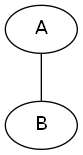
\includegraphics[width=.9\linewidth]{dotResult.png}
\end{center}

\section{R}
\label{sec:orgb034b28}

\subsection{Just run some R code in a new session}
\label{sec:org3d6d0ea}

\begin{verbatim}
print("HI MOM")
\end{verbatim}

\begin{verbatim}
[1] "HI MOM"
\end{verbatim}

\subsection{Access a table in this document as a data.frame}
\label{sec:org09ef2fc}

\begin{verbatim}
someData
\end{verbatim}

\begin{verbatim}
  factor.1 factor.2 value.1 value.2
1        a        z       1       5
2        a        x       2       6
3        a        y       3       7
4        b        x       4      NA
\end{verbatim}

\subsection{Output from R as a org-mode table}
\label{sec:org7b70929}

\begin{verbatim}
someData
\end{verbatim}

\begin{center}
\begin{tabular}{llrr}
a & z & 1 & 5\\
a & x & 2 & 6\\
a & y & 3 & 7\\
b & x & 4 & nil\\
\end{tabular}
\end{center}

\subsection{Run some code in a R persistent session (the someData variable is available for later blocks)}
\label{sec:orgfeced25}
\begin{verbatim}
someData <- data.frame(a=1:10, b=rnorm(10))
print(someData)
\end{verbatim}

\begin{verbatim}
    a            b
1   1  0.379789874
2   2  1.998294645
3   3  0.466352572
4   4  0.001298143
5   5 -1.656637383
6   6 -1.037567358
7   7 -1.107296046
8   8 -1.653000457
9   9 -0.889483086
10 10 -0.387415308
\end{verbatim}

\subsection{Use the someData variable in the session, and draw a graph.}
\label{sec:org7dc2771}

No speical org-mode stuff for graphics.  Just saved the output in files via R.  Add link text later.

\begin{verbatim}
g <- ggplot(someData, aes(x=a, y=b)) + geom_line()
ggsave("rOut1.png", width=8, height=6, dpi=100, units='in', plot=g);
ggsave("rOut1.pdf", width=8, height=6, dpi=600, units='in', plot=g);
\end{verbatim}

The graph:

\begin{center}
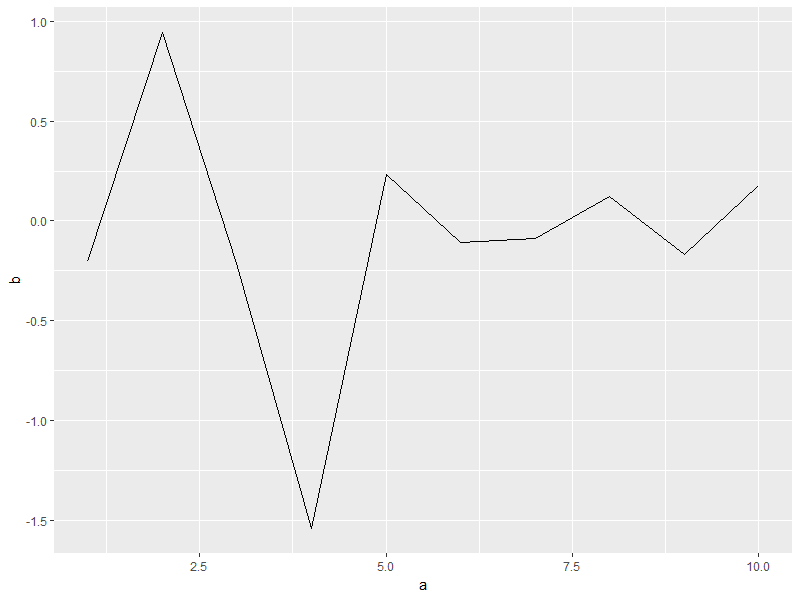
\includegraphics[width=.9\linewidth]{rOut1.png}
\end{center}

A high quality PDF version is \href{rOut1.pdf}{here} -- note the "here" is a link for both \LaTeX{} and HTML.

\subsection{We can use org-mode to make the file too.}
\label{sec:org51b49a9}

Note: :session is required for this to work -- otherwise we must "print" the graphic.

\begin{verbatim}
ggplot(someData, aes(x=a, y=b)) + geom_line()
\end{verbatim}

\begin{center}
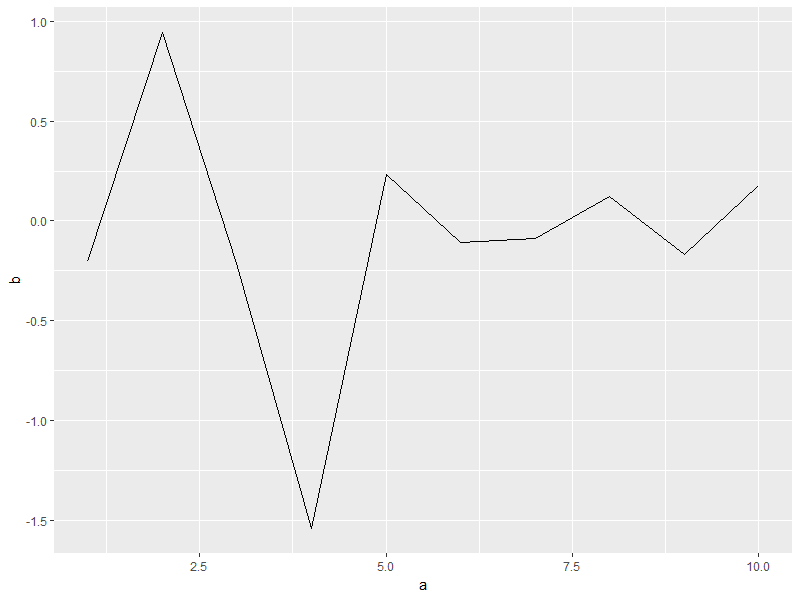
\includegraphics[width=.9\linewidth]{rOut1.png}
\end{center}

\subsection{And plotly works too}
\label{sec:org939eba7}

Note the silent output -- we don't need the result, so we just don't print it.

\begin{verbatim}
library(plotly)
library(htmlwidgets)
data(diamonds, package = "ggplot2")
ggp <- ggplot(diamonds, aes(x = log(carat), y = log(price))) + geom_hex(bins = 100)
plp <- ggplotly(ggp)
saveWidget(plp, "examplePlotly.html", selfcontained=FALSE, libdir="examplePlotlyLib")
\end{verbatim}

\section{Reproduciblity}
\label{sec:org4fc55ae}

This section is here to help anyone wishing to reproduce the results above, or to understand the mechanics of how the results were obtained..

Reminder: All blocks in the entire tree can be evaluated with C-C C-V C-S

\subsection{FILES}
\label{sec:org9944178}

Documented in this section are (for each file in this archive):

\begin{itemize}
\item SHA1
\item Output from an 'ls -l' command
\item Output from the 'wc' command -- byte, word, and line counts
\end{itemize}

The use cases are two fold:

\begin{itemize}
\item Insure that the input data files being used are the same
\item Check if reproduced results match
\end{itemize}

Replace the \texttt{`find ./ -type f`} with a list of files and/or wildcards to explicitly select the desired files.

\begin{verbatim}
date
for c in wc 'openssl sha1' 'ls -l' ; do
    echo $c; $c `find ./ -type f`
done
\end{verbatim}

\subsection{ENVIRONMENT}
\label{sec:org0e2ba9d}

The input files are only part of the reproduciblity equation.  It is also important to understand the tools and computational environment used for the
original analysis.  This section contains various bits of meta-data about the tools and system I used for this analysis.

\subsubsection{Embedded Ruby Version}
\label{sec:org2c45e38}

\begin{verbatim}
puts(RUBY_VERSION)
\end{verbatim}

\subsubsection{Embedded Perl Version}
\label{sec:orga805d34}

\begin{verbatim}
print $]
\end{verbatim}

\subsubsection{Embedded R Information}
\label{sec:org3bcd215}

\paragraph{R version}
\label{sec:org24bb25a}

\begin{verbatim}
R.version
\end{verbatim}

\paragraph{Session Information}
\label{sec:org13bd9bb}

\begin{verbatim}
sessionInfo()
\end{verbatim}

\paragraph{Loaded Package Versions}
\label{sec:org91da9ed}

\begin{verbatim}
installed.packages()[(loadedNamespaces()),c('Version', 'LibPath')]
\end{verbatim}

\subsubsection{Emacs Information}
\label{sec:org0a222f9}

\paragraph{Emacs Version}
\label{sec:org8d3cab5}

\begin{verbatim}
(emacs-version)
\end{verbatim}

\paragraph{org-mode Version}
\label{sec:orga084460}

\begin{verbatim}
org-version
\end{verbatim}

\paragraph{ESS Version}
\label{sec:orgbe44650}

\begin{verbatim}
(ess-version)
\end{verbatim}

\paragraph{Process Environment}
\label{sec:orgcf62915}

\begin{verbatim}
process-environment
\end{verbatim}

\paragraph{System Type}
\label{sec:orgb405fe4}

\begin{verbatim}
system-type
\end{verbatim}

\paragraph{System Configuration}
\label{sec:org2bfafe6}

\begin{verbatim}
system-configuration
\end{verbatim}

\subsubsection{System Information}
\label{sec:orga551ffa}

\begin{verbatim}
for e in date whoami groups id hostname domainname dnsdomainname 'ifconfig -a' 'uname -a' 'openssl version' locale 'ldconfig -p' 'dpkg-query -l'; do
  c=`echo $e | awk '{print $1}'`;
  if hash $c 1>/dev/null 2>/dev/null; then 
    ruby -e 'puts("="*90)'
    echo $e
    sh -c "$e"
  fi
done
\end{verbatim}

\subsubsection{Command Line Tool Information}
\label{sec:org9cfac48}

\begin{verbatim}
for e in gcc g++ gfortran                               \
         wc ls grep sed awk cut sort uniq               \
         bash ksh tcsh dash csh sh zsh                  \
         vi vim emacs em                                \
         ruby ruby1.8 ruby2 python3 python2 perl        \
         gnuplot maxima octave M2 gap julia R           \
         qtiplot ggobi                                  \
         povray                                         \
         openscad xcircuit                              \
         convert pqiv import display                    \
         gs pdftex pdflatex tex latex dvips             \
         sbcl clisp ecl ccl                             \
         diff diff3 patch merge                         \
         sqlite3 mysqld                                 \
         paraview visit                                 \
         grass                                          \
         tar gzip bzip2 ; do
  ruby -e 'puts("="*90)'
  echo "Tool: $e"
  if hash $e 1>/dev/null 2>/dev/null; then 
    CPH=`which $e`
    if [ -n "$CPH" -a -e "$CPH" ] ; then
      echo $CPH    | sed 's/^/  Path: /'
      ls -ld $CPH  | sed 's/^/  ls-l: /'
      $e --version | sed 's/^/  Ver:  /'
    else
      echo "  Unable to locate (which): $e"
    fi
  else
    echo "  Unable to locate (hash): $e"
  fi
done
ruby -e 'puts("="*90)'
\end{verbatim}

\section{Publishing}
\label{sec:orgfeb8b3b}
By "publishing" I mean simply copying stuff from the current directory tree to a new location -- usually one shared by a web/file server or to a staging area
to be later uploaded to a web server.

To control very precicely what gets published, put the files in the file \url{files\_to\_publish}.  One way to do that is like so:

\begin{verbatim}
EXT2PUB='.org .html .png .gif .jpeg .pdf .ps .sh .rb .R .c .cpp .h .hpp .csv .csv.gz'
if test -e files_to_publish; then cp files_to_publish files_to_publish_before; wc -l files_to_publish_before; fi
for e in $EXT2PUB; do
  find ./ -name "*$e"
done | sed 's/^\.\///' | egrep -v '^(#|\.)' > files_to_publish
sort files_to_publish | uniq > files_to_publish~
mv files_to_publish~ files_to_publish
wc -l files_to_publish
\end{verbatim}

\begin{verbatim}
PUB_DIR=/tmp/foo
HTML_NAME=
PUB_MODES=a+rX
VERBOSE=-ii
if test -z "$HTML_NAME" -o 0 -eq `find ./ -cnewer "$HTML_NAME" -a -type f 2>/dev/null | wc -l `; then
    RSYNC_OPTS='--delete -a'
    if test -n "$VERBOSE";         then RSYNC_OPTS="$RSYNC_OPTS $VERBOSE"; fi
    if test -e '.rsync-filter';    then RSYNC_OPTS="$RSYNC_OPTS -F"; fi
    if test -e 'files_to_publish'; then RSYNC_OPTS="$RSYNC_OPTS --files-from=files_to_publish"; fi
    date
    rsync $RSYNC_OPTS ./ "$PUB_DIR"
    date
else
  echo "ERROR: $HTML_NAME is not the newest file here.  Please regenerate it (C-c C-e h h)!"
fi
\end{verbatim}
\end{document}
